\documentclass[10pt,onecolumn,a4paper]{article}


\usepackage{fancyhdr}
\usepackage{multicol}
\usepackage{array}
\usepackage{multirow}
\usepackage{graphicx, geometry}
\usepackage[english, russian]{babel}
\usepackage{blindtext}
\usepackage{amsmath}
\usepackage{colortbl}
\newgeometry{left=0.8cm,right=0.8cm,bottom=0.1cm,top=1cm}
\begin{document}
\begin{center}
\large Федеральное государственное автономное образовательное учреждение высшего образования «Национальный исследовательский университет ИТМО»\\
Факультет Программной Инженерии и Компьютерной Техники\\
\hfill 


\vspace{7cm}
\Large Лабораторная работа №6 \\
Работа с системой компьютерной вёрстки T\raisebox{-0.3em}{E}X\\
Вариант: 106\\
\end{center}

\vspace{7.5cm}
 
\begin{flushright}
\textit{Выполнил:}\\
Шмунк Андрей Александрович\\
Группа P3108\

\textit{Проверил:}\\
Доцент ПИиКТ, кандидат технических наук\\
Балакшин Павел Валерьевич\\
\end{flushright}
 
\vfill

\begin{center} Санкт-Петербург, 2023 \end{center}

\thispagestyle{empty}
\newpage
\begin{center}
    Информация
\end{center}
\begin{multicols}{3}
\noindent сообщено не позднее 1 августа 2000 года.
Тетрадь с выполненными заданиями (по физике и математике) высылайте по адресу: 141700
\emph{г.Долгопрудный Московской области, Институтский пер., 9, МФТИ, ЗФТШ.}

Для учащихся Украины работает Киевский филиал ЗФТШ при МФТИ. Желающим поступить следует высылать работы по адресу: 252680 г.Киев, пр. Вернадского, д.36, Институт ме- таллофизики, Киевский филиал ЗФТШ при МФТИ. Телефон: (044) 444-95-24.

Для учащихся из стран ближнего зарубежья возможно платное обуче- ние на заочном и очно-заочном отделениях ЗФТШ. Условия обучения для прошедших конкурсный прием будут сообщены дополнительно.

Ниже приводятся вступительные задания по физике и математике. В зада- нии по физике: задачи 1 - 5 предназ- начены для учащихся седьмых клас- сов, 3—8 – для восьмых классов, 6 - 11 – для девятых классов, 10 - 16 - для десятых классов. В задании по математике: задачи 1—5 предназна- чены для учащихся седьмых классов, 2—8 – для восьмых классов, 5—11 – для девятых классов, 8 - 14 – для десятых классов. Номера классов указаны на текущий 1999/2000 учебный год.
\begin{center}
Вступительное задание по математике
\end{center}

\textbf{1.} Дома Винни-Пуха и Пятачка на- ходятся на расстоянии 1 км друг от друга. Однажды они одновременно вышли из своих домов, и каждый пошел в каком-то направлении по прямой. Винни-Пух проходил 3 км в час, а Пятачок – 4 км в час. Через некото- рое время они встретились. Сколько времени могло продолжаться их путешествие? Укажите наибольшее и наименьшее время.

\textbf{2.} Внутри острого угла отмечена точка А. Найдите на сторонах угла точки В и С такие, чтобы периметр треугольника АВС был наимень- шим.

\textbf{3.} Имеются три сосуда емкостей 3л,3ли7л.Можноли,пользуясь этими сосудами, налить в большой сосуд ровно 5 л воды?
Найдите все пятизначные числа вида
\begin{right}

$2m57n=2*10^4++m*10^3+4*10^2+7**10+n$

(m и n - цифры,  которые делятся на 15)
\end{right}

\textbf{5.} На плоскости даны три прямые а, b и с, не проходящие через одну
точку. Постройте на прямых а и b точки А и В так, чтобы отрезок АВ был перпендикулярен прямой с и де- лился этой прямой пополам.

\textbf{6.} Числа х, у, z – последовательные члены арифметической прогрессии, их сумма равна 21.Числах –1,у+1, z + 21 являются последовательными членами некоторой геометрической прогрессии. Найдите числа х, у, z.

\textbf{7.} Решите уравнение
\begin{center}
$\sqrt{2-x}=|x-1|-2$
\end{center}
\textbf{8.}В корзине лежало не более 70 грибов. После разбора оказалось, что 52\% из них – белые. Если отложить три самых маленьких гриба, то среди оставшихся будет ровно половина белых. Сколько грибов было в корзине?

\textbf{9.}Острый угол АВС ромба ABCD равен 60°. Окружность проходит через точку пересечения диагоналей ромба, касается прямой АВ в точке В и пере- секает сторону CD в точке Е. Определите, в каком отношении точка Е делит отрезок CD.

\textbf{10.}Множество А состоит из всех точек плоскости, координаты (х; у) которых удовлетворяют системе неравенств
\[\begin{cases}
x^2+(a+4)x+4a\leq a ,\\
3x+y-(2a+4)\leq 0.
\end{cases}
\]
Определите, при каких значениях параметра а множество А содержит отрезок [–2; –1] оси Ох.

\textbf{11.}Решите неравенство
\begin{center}
$\frac{10-3x+\sqrt{x^2+x-6}}{4-x}\geq1$
\end{center}

\textbf{12.}Точки K и L являются середина- ми боковых сторон АВ и ВС равнобед- ренного треугольника АВС. Точка М расположена на медиане AL так, что АМ:ML=13:12.Окружностьс центром в точке М касается прямой АС и пересекает прямую KL в точках Р и Q. Найдите периметр треугольника АВС,еслиKL=10,PQ=4.

\begin{left}
\textbf{13.}Решите систему уравнений
\end{left}
\[\begin{cases}
17 \cos{2x} - 7 = 21\sin{x}*\cos{2y},\\
\cos{x}=\sqrt{3\sin{x}}*\cos{y}.
\end{cases}
\]

\textbf{14.}На координатной плоскости рассматривается фигура Ф, состоящая из всех точек, координаты (a; b) которых таковы, что система уравнений
\[\begin{cases}
ax+by=1,\\
3x+ay=-1,\\
(a-1)x+(b+2)=-2.
\end{cases}
\] 
имеет решение. Изобразите фигуру Ф и составьте уравнения всех прямых, каждая из которых проходит через точку (4; 3) и имеет с фигурой Ф единственную общую точку.

\begin{center}
Вступительное задание по физике
\end{center}

\textbf{1.}Автомобиль первую треть пути ехал со скоростью v1 = 30 км/ч, оставшуюся часть пути он ехал со скоростью, в два раза большей средней скорости на всем пути. Найдите скорость автомобиля на второй части пути.

\textbf{3.}Труба массой m = 100 кг лежит на земле. Какую минимальную силу F надо приложить к концу трубы, чтобы его приподнять?

\textbf{3.}С вертолета сфотографирован пароход, идущий по озеру курсом на север. На фотографии (рис.1) запе-

\begin{center}
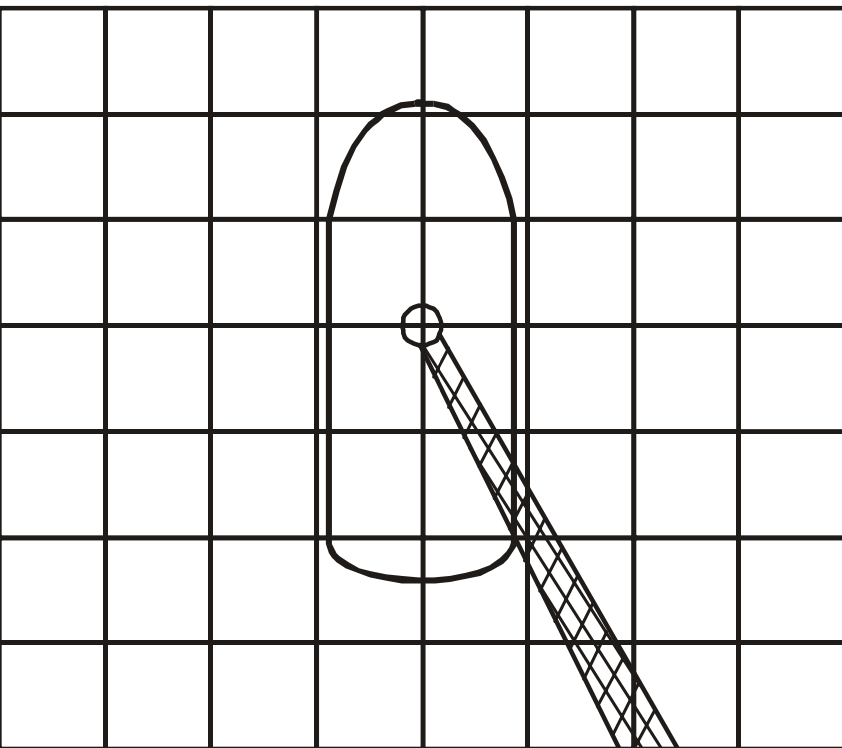
\includegraphics[width=0.25\textwidth]{ris1}

\caption{Рис. 1}
\end{center}

чатлен шлейф дыма от парохода. Определите по фотографии скорость па- рохода, если съемка проводилась при юго-западном ветре, скорость которого v=5м/с.

\textbf{4.}В два цилиндрических сообщаю- щихся сосуда наливают ртуть. Пло- щадь сечения одного из сосудов вдвое больше площади сечения другого. Широкий сосуд доливают водой до края. На какую высоту h поднимется при этом уровень ртути в другом со- суде? Первоначально уровень ртути был на расстоянии l от верхнего края сосуда. Плотности ртути ρ и воды ρ0 известны.

\textbf{5.}В сосуде с водой плавает кусок льда, удерживаемый нитью (рис.2). Сила натяжения нити F = 10 Н. На

\begin{center}
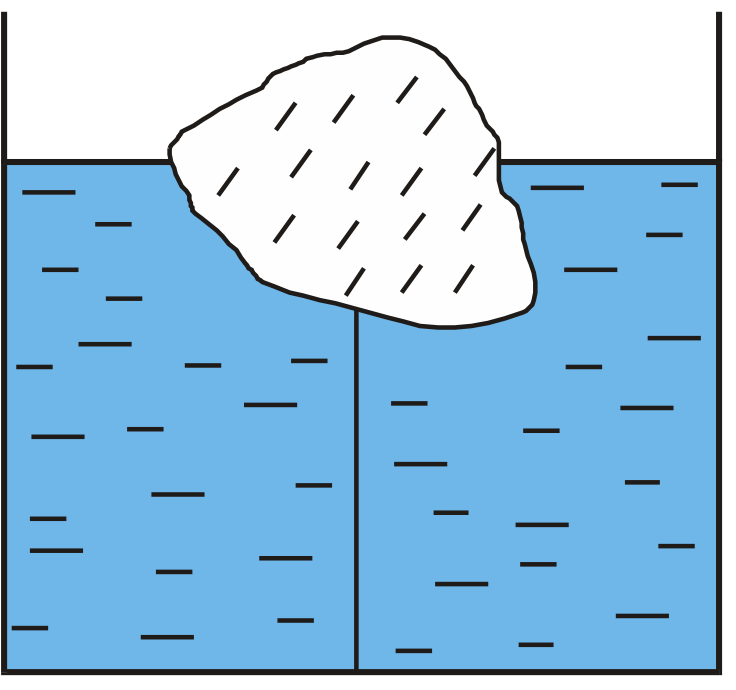
\includegraphics[width=0.25\textwidth]{ris2}


\caption{Рис. 2}
\end{center}

\end{multicols}
\newgeometry{left=0.8cm,right=0.8cm,bottom=0.1cm,top=2cm}
\thispagestyle{fancy}
\fancyhead{} 
\fancyhead[C]{\LargeМАТЕМАТИЧЕСКИЙ КРУЖОК}
\begin{center}
\begin{tabular}{  m{12cm} m{7cm} } 
\begin{center}
\huge\textbf{Странные игроки}

\normalsize\textit{\textbf{Б.ФРЕНКИН}}\end{center}\hrule&Решение. а) Пусть в турнире шесть участников (см. таблицу). Первые трое сыграли между собой вничью, четвертый с пятым – также вничью, причем проиграли первым троим, а шестой выиграл у первых трех и проиграл четвертому и пятому. Тогда шестой разделил первое место с первыми тремя игроками и при этом является странным.

\end{tabular}
\end{center}
\begin{tabular}{  m{5.8cm}  m{5.6cm} m{7.2cm}}

\small{\textbf{Парадоксы турнирных таблиц}
Спортивные турниры служат источ- ником множества логических задач. Даже при простой схеме проведения легко возникают необычные ситуации.
    
    

\quad\textbf{Пример.} \textit{Тридцать три богатыря устроили соревнования по борьбе. Каждый боролся с каждым один раз. Победа давала 1 очко, поражение – 0, ничьих не было. Один богатырь выступил странно. Он победил всех, кто в итоге набрал больше очков, чем он, и проиграл всем, кто набрал меньше, чем он. Равного с ним коли- чества очков не набрал никто. Докажите, что странный богатырь занял место не выше тринадцатого и не ниже двадцать первого.}

\quad\textbf{Решение.} Предположим, что странный богатырь занял место выше тринадцатого. Количество тех, кто набрал меньше очков, превышает двадцать. Рассмотрим их поединки между собой. Каждый из них провел не менее 20 поединков. Кто-то выиграл не менее половины этих поединков и, следовательно, набрал в них не менее 10 очков. Кроме того, он победил странного – значит, всего получил не менее 11 очков. Странный богатырь набрал больше его, т.е. не менее 12 очков. Но странный победил только тех, кто выше его в турнирной таблице – следовательно, их не менее 12, и странный не мог занять место выше тринадцатого.

\quadПоменяем теперь результаты всех матчей на противоположные. Условия задачи по-прежнему выполняются, а последовательность занятых мест изменилась на об- ратную. Странный богатырь занял теперь место не выше тринадцатого. Остается 
заметить, что при 33 участниках двадцать первое место – это тринадцатое с конца.

\quadНа любом турнире возможен странный участник вроде такого богатыря. Изучим эту ситуацию подробнее: в ней кроется немало интересного.

\quadИтак, странный участник кругового турнира характеризуется тем, что он выиграл у всех, кто набрал больше очков, чем он, и проиграл всем, кто набрал меньше. С теми, кто выступил наравне с ним, такой игрок мог сыграть как угодно. Подразумевается, что турнир проходит в один круг, причем победа дает одно очко, ничья – половину, поражение – ноль.}

&\small{Число участников турнира далее обозначаем N. Результат игрока – это сумма очков, которую он набрал.
Однако такое определение странного игрока имеет некий изъян. А именно, пусть все участники турнира получили поровну. Тогда для каждого из них отсутствуют и набравшие больше, и набравшие меньше. Формально мы можем считать всех игроков странными. Но это само по себе странно, особенно в такой тривиальной ситуации. Поэтому в дальнейшем всегда предполагается, что \textit{не все участники турнира набрали одинаковое количество очков}. При этом считается допустимым, если никто не на- брал больше очков, чем странный игрок. Точно так же ему не запрещается разделить и последнее место.

\begin{center}
    \textbf{\largeГде искать странных?}
\end{center}

Представьте себе таблицу результатов турнира. Где в ней могут располагать- ся странные игроки? Для начала дока- жем следующий факт:

\quad\textbf{Задача 1.} \textit{Все странные участники имеют одинаковое количество очков.}

\quad\textbf{Решение.} Пусть А и Б – странные, причем А набрал больше очков, чем Б. Тогда А проиграл Б. Очевидно, А сыграл с каким-то третьим игроком (и не с одним) лучше, чем с ним сыграл Б. Но если такой игрок В набрал меньше очков, чем А, то В выиграл у А (по определению странного игрока). Если же В набрал не меньше очков, чем А, то В набрал больше, чем Б, и тогда Б (как странный) выиграл у В. Значит, А ни с кем не сыграл лучше, чем Б, в противоречии с предыдущим.

\quadЕсли игрок получил столько же очков, сколько и странные, но сам не является странным, то назовем его \textit{средним}. Тех, кто набрал больше, будем называть \textit{сильными}, а тех, кто набрал меньше, – \textit{слабыми}.

\quadВ какой же части турнирной таблицы располагаются странные? Например:
Задача 2. а) Может ли странный игрок разделить первое место? А пос- леднее?
б) Могут ли на первом или последнем месте находиться только странные?
}



&
\normalsize{
\begin{center}
\begin{tabular}{ c | c | c | c | c | c | c | }

 \multicolumn{1}{c}{}& \multicolumn{1}{c}{1} & \multicolumn{1}{c}{2} & \multicolumn{1}{c}{3} & \multicolumn{1}{c}{4} & \multicolumn{1}{c}{5} & \multicolumn{1}{c}{6} \\
 \cline{2-7}
 1 &\cellcolor[gray]{0.8} & $\frac{1}{2}:\frac{1}{2}$ & $\frac{1}{2}:\frac{1}{2}$ & $1:0$ & $1:0$ & $0:1$ \\[1ex]
 \cline{2-7}
 2& $\frac{1}{2}:\frac{1}{2}$ &\cellcolor[gray]{0.8} & $\frac{1}{2}:\frac{1}{2}$ & $1:0$ & $1:0$ & $0:1$ \\[1ex]
 \cline{2-7}
 3 & $\frac{1}{2}:\frac{1}{2}$ & $\frac{1}{2}:\frac{1}{2}$ &\cellcolor[gray]{0.8} & $1:0$ & $1:0$ & $0:1$ \\[1ex]
 \cline{2-7}
 4& $0:1$ & $0:1$ & $0:1$ & \cellcolor[gray]{0.8} & $\frac{1}{2}:\frac{1}{2}$ & $1:0$ \\ [1ex]
 \cline{2-7}
 5 &  $0:1$ &  $0:1$ &  $0:1$ & $\frac{1}{2}:\frac{1}{2}$ & \cellcolor[gray]{0.8}& $1:0$\\[1ex]
 \cline{2-7}
 6 & $1:0$ & $1:0$ & $1:0$ & $0:1$ & $0:1$ &\cellcolor[gray]{0.8} \\[1ex]
 \cline{2-7}

\end{tabular}
\end{center}
\quadЧтобы поместить странного игрока на последнее место, поменяем все результаты на противоположные.

\quadб) Пусть первое место полностью при- надлежит странным, и их число равно М. Любой из них проиграл всем, кто не делит первое место, и поэтому набрал не более М – 1 очков. Игрок, не находящийся на первом месте, выиграл у всех странных и потому получил результат не меньше М, что противоречит предыдущему. Значит, первое место не может принадлежать только странным.

\quadДля последнего места рассуждение аналогичное.
\newline
\quadМы видели, что все странные на- бирают одинаковое количество очков. И не нужно знать исход каждого матча, чтобы определить это количе- ство:
\quad\textbf{Задача 3.}\textit{ Известны результаты всех игроков. Известно также, что на турнире были странные участни- ки. Как определить, сколько очков они набрали?}
\newline
Решение этой задачи, а также задач 4, 5 и 7 см. в конце журнала.
\begin{center}
\textbf{\large{Обычных – всегда большинство. Но не всегда подавляющее}}
\end{center}


Сколько же может быть на турнире странных участников? Ясно, что все одновременно такими не бывают. Бо- лее точно:

\quad\textbf{Задача 4.} \textit{ а) Число странных всегда не больше [N/2] — 1. Докажите это.}
}
\newline
\newline
\newline
\newline
\newline
\newline
\newline
\newline
\newline
\end{tabular}
\end{document}
